
\chapter{Finite Games}\label{chapter:finiteGames}

\section{Definition}\label{section:definition}

\begin{itemize}
    \item Nice definitions in \cite{mertikopoulos} p. 470. Make sure to include Mixed Extensions of Finite Games (Ex.2.1)
    \item Also nice one in \cite{flokas} p.4
    \item also include the notion of regret in terms of finite games as in \cite{mertikopoulos} p.466 Introduction
    \item also need to rephrase Online Mirror Descent into Ascent algorithms as we are maximizing payoffs
\end{itemize}


\section{Equilibria Concepts}\label{section:equilibriaConcepts}

\begin{itemize}
    \item Define MNE, PNE, CE, CCE (e.g. NE in \cite{mertikopoulos} 2.2)
    \item note that Computing NE is PPAD hard
    \item No regret dynamics converge to the game's set of CCE. \cite{jafari} or \cite{flokas} p.2
    \item CCE is a weak concept, because it may contain strictly dominated (pure) strategy profiles with positive probability. CCE is learnable but weak. (ComputingBNE, p.3)
    \item define Strict vs. Weak Nash Equilibrium
    \item mention that MNE cannot be strict
    \item No-regret algorithms are known to converge to converge to the Nash Equilibrium in games for which PNE exists.\cite{jafari} 4.1. (need to be more concrete here as in \cite{mertikopoulos} only strict NE survive)
    \item Under FTRL dynamics only strict NE survive \cite{flokas} Theorem 2 p.3
    \item There exist no uncoupled dynamics which guarantee Nash Convergence. Hart, Mas-Colell impossibility result \cite{hart}
\end{itemize}

\section{Variational Stability}\label{section:variationalStability}

\begin{itemize}
    \item Define as in \cite{mertikopoulos} 2.3 Variational stability p.473
    \item No interior of the strategy space can be asymptotically stable under FTRL \cite{flokas} Theorem 1 p.2
    \item That implies that MNE can not be stable
    \item When NE is not strict FRTL is not stable \cite{flokas} abstract
    \item asymptotically stable is defined as both stable and attracting \cite{flokas} 4.1 p.8
    \item If asymptotically stable then PNE \cite{flokas} Theorem 2
    
    \item stable equilibria are locally attracting with high probability \cite{mertikopoulos}, Abstract, Theorem 4.11 (local convergence of local stable equilibria with high probability) 
    \item globally stable equilibria are globally attracting with probability 1 \cite{mertikopoulos}, Abstract. Already refer to Prisoner's Dilemma in \ref{subsection:prisonersDilemma}
    \item If x* globally stable then x* is unique NE \cite{mertikopoulos} Prop. 2.5 
    \item the following are equivalent: \cite{mertikopoulos} Prop. 5.2
    \item x* is a strict NE
    \item x* is stable
    
    
    \begin{figure}
    \centering
    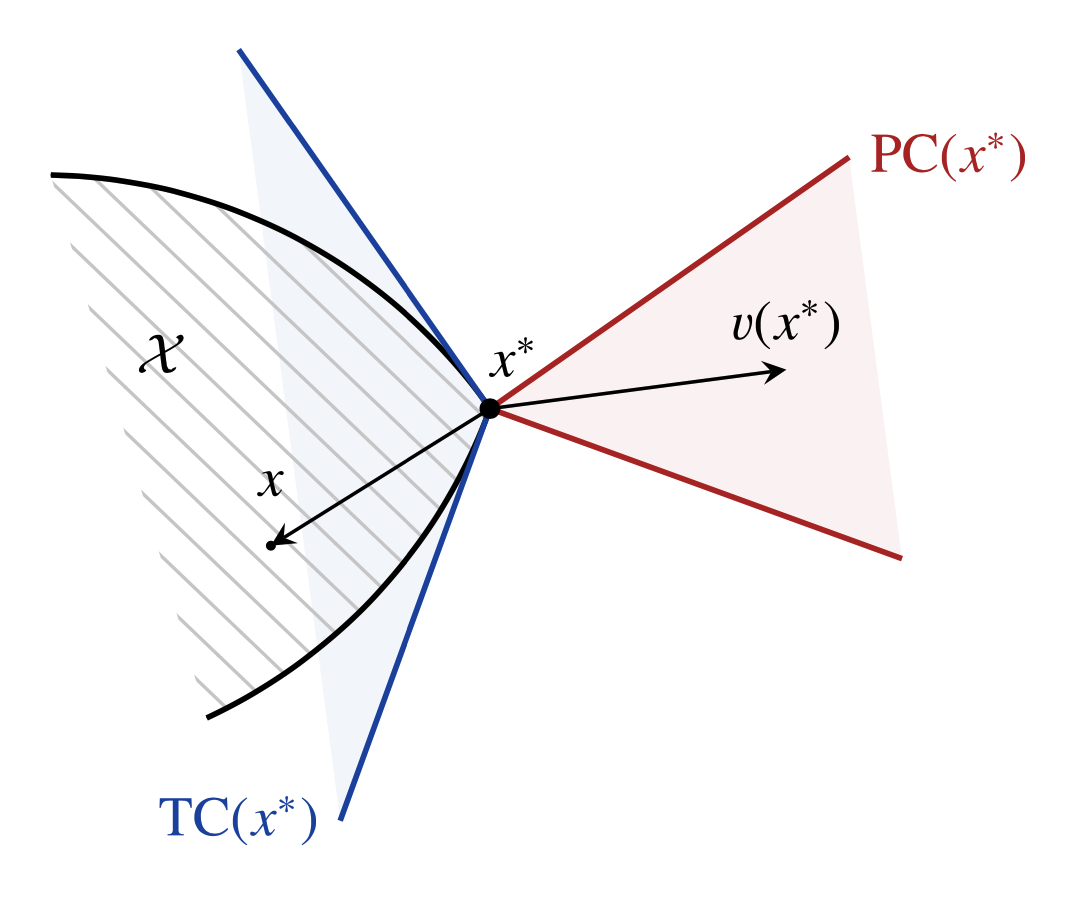
\includegraphics[width=0.5\textwidth]{logos/Mertikopoulos-VS.png}
    \caption{...}
    \label{Mertikopoulos-VS}
    \end{figure}

\end{itemize}

